\documentclass[11pt, a4paper]{extarticle}
\setlength{\parskip}{0.5em}

%%% Работа с русским языком
\usepackage{cmap}					% поиск в PDF
\usepackage{mathtext} 				% русские буквы в формулах
\usepackage[T2A]{fontenc}			% кодировка
\usepackage[utf8]{inputenc}			% кодировка исходного текста
\usepackage[english,russian]{babel}	% локализация и переносы
\usepackage{mathtools}   % loads »amsmath«
\usepackage{graphicx}
\usepackage{caption}
\usepackage{physics}
\usepackage{subcaption}
\usepackage{tikz}

\usepackage{hyperref}
\hypersetup{urlcolor=cyan,  colorlinks=true, linkcolor=cyan}

%%% Дополнительная работа с математикой
\usepackage{amsmath,amsfonts,amssymb,amsthm,mathtools} % AMS
\usepackage{icomma} % "Умная" запятая: $0,2$ --- число, $0, 2$ --- перечисление

%% Шрифты
\usepackage{euscript}	 % Шрифт Евклид
\usepackage{mathrsfs} % Красивый матшрифт

\newcommand{\code}[1]{{\color{blue} #1}}
\newcommand{\form}[1]{{\color{magenta} #1}}

\title{Инструкция по переводу .Rmd-файлов в формат \LaTeX-Beamer}
\author{VMarco}
\date{\today}

\usepackage{geometry}
\geometry{
	a4paper,
	left=20mm,
	top=20mm,
	right=20mm
}
\setlength{\parindent}{0cm}
\let\P\relax
\DeclareMathOperator{\P}{\mathbb{P}}
\DeclareMathOperator{\E}{\mathbb{E}}

\begin{document}
	
\maketitle

\renewcommand{\abstractname}{\vspace{-\baselineskip}}
\begin{abstract}
	Инструкция основана на примере промежуточного экзамена 2017-го года. В тексте использованы следующие цветовые обозначения:
	\begin{description}
		\item[\code{Синим}] обозначены фрагменты кода в RStudio или в редакторе \LaTeX.
		\item[\form{Розовым}] обозначены названия программ, форматы и названия файлов и пакетов, кнопок – всё, что относится к коду, но им не является.
	\end{description}
	Все используемые в инструкции файлы c кодом доступны по \href{https://github.com/V-Marco/rexamsconverter}{ссылке}. По этой \href{https://github.com/bdemeshev/probability_hse_exams/tree/master/tests}{ссылке} можно найти использованные материалы. 
\end{abstract}

\tableofcontents
\newpage

\section{Необходимые файлы}

\begin{enumerate}
	\item Папка с файлами \form{.Rmd}, в формате <<\form{Номер\_задания.Rmd}>> (Рис. 1).
	\begin{figure}[h!]
		\centering
		\fbox{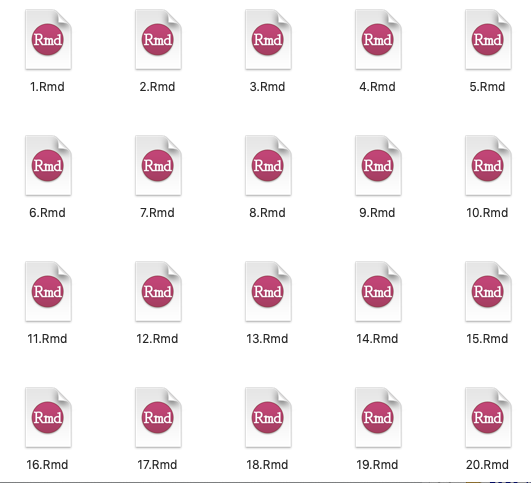
\includegraphics[width=0.8\linewidth]{1.png}}
		\caption{Содержимое папки с файлами}
	\end{figure}

	Каждый файл \form{.Rmd} должен быть в формате пакета \form{rexams} (Рис. 2).
	\begin{figure}[h!]
		\centering
		\fbox{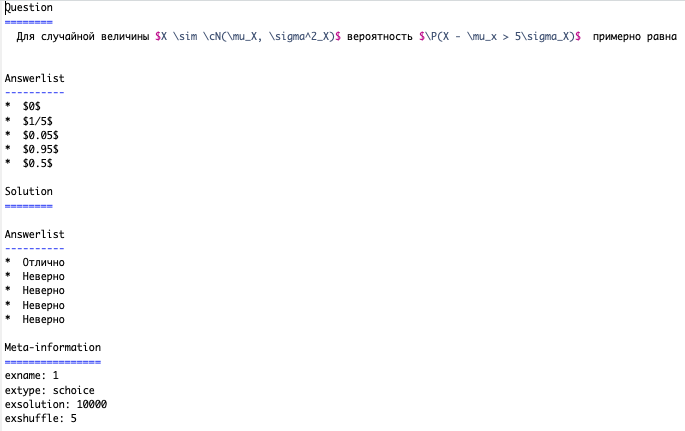
\includegraphics[width=0.8\linewidth]{2.png}}
		\caption{Пример файла .Rmd в нужном формате}
	\end{figure}

	\item \form{rmdExams2beamerlatex.R} – переводит файлы \form{.Rmd} в формат \LaTeX-Beamer. Чтобы скачать файл с GitHub из браузера, нажмите на него правой кнопкой мыши и выберите <<Скачать файл по ссылке>>.
	\item \form{RStudio} с установленным пакетом \form{readr} (в инструкции будет использоваться \form{RStudio} на английском языке).
	\item Настроенный \LaTeX \,(в инструкции будет использоваться программа \form{TexStudio}).
\end{enumerate}

\section{Создание и компиляция файла \LaTeX-Beamer}
\begin{enumerate}
	\item Откройте в \form{RStudio} файл \form{rmdExams2beamerlatex.R} и загрузите в память функцию \\ \code{RmdExams2beamerlatex}. Для этого выделите всё, что есть в файле, и нажмите кнопку \form{Run}. Если всё сделано верно, то на правой панели в окне \form{Functions} появится \form{RmdExams2beamerlatex}, а в нижней панели, в консоли, появится синий текст.
	
	\item Установите в качестве \form{Working Directory} папку, в которой находится папка с \form{.Rmd} файлами. Это удобно сделать через правую нижюю панель, где представлена навигация по папкам. Используя окно навигации, перейдите в папку, в которой находится папка с \form{.Rmd} файлами. Нажмите на кнопку \form{More} (с шестерёнкой) и выберите \form{Set As Working Directory}. Если всё сделано верно, то в консоли появится надпись синим текстом: \code{setwd(путь к папке)}.
	
	\item Наберите в консоли: \code{RmdExams2beamerlatex('название папки, в которой лежат файлы .Rmd')}. Не забудьте кавычки. Например, в нашем случае папка называется \form{2017\_midterm\_rmd}, поэтому в консоль следует ввести \code{RmdExams2beamerlatex('2017\_midterm\_rmd')}. Если всё сделано верно, то функция исполнится без ошибок, и в консоли будет выполнен переход на новую строку. Красных надписей не появится. После этого шага коносль должна выглядеть примерно так (Рис. 3).
	
	\begin{figure}[h!]
		\centering
		\fbox{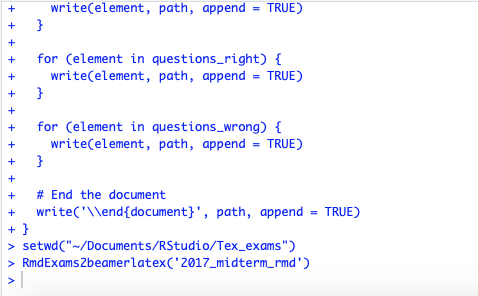
\includegraphics[width=0.8\linewidth]{3.png}}
		\caption{Консоль после шага 3.}
	\end{figure}
	
	После этого шага \form{RStudio} можно закрыть. 
	
	\item Зайдите в папку, в которой находятся файлы \form{.Rmd}. В ней должен появиться файл \form{exam.txt}. Если хотите, переместите его в любую другую папку и переименуйте. Измените разрешение файла с \form{.txt} на \form{.tex}. Откройте файл в программе для работы с файлами \form{.tex} (в инструкции используется \form{TexStudio}).
	
	\item Далее необходимо попробовать скомпилировать файл. При первом запуске появится уведомление о множестве ошибок. Необходимо последовательно исправить их все (советы смотрите ниже). В основном, ошибки появляются в тех местах, где в синтаксисе \LaTeX \,присутствуют фигурные скобки \code{\{$\cdot$\}} – дроби, конструкции \code{cases} и проч.
	
	\textbf{Важно:} \form{.tex} файл можно разбить на три структурно-смысловые части: сначала подряд идут сами вопросы (их можно опознать по команде \code{$\backslash$label\{номер вопроса\}} перед началом каждого слайда), затем – слайды, показывающие, что ответ на конкретный вопрос верный (\code{$\backslash$label\{номер вопроса-Yes\}}), затем – что неверный (\code{$\backslash$label\{номер вопроса-No\}}). Соответственно, сам текст вопроса повторяется три раза (смотрите Рис. 4-6). При исправлении следует скорректировать все три текста вопроса. 
	
	\begin{figure}[h!]
	\centering
	\fbox{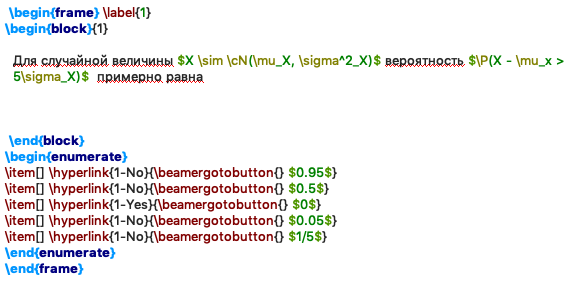
\includegraphics[width=0.8\linewidth]{4.png}}
	\caption{Текст вопроса номер 1.}
	\end{figure}

	\begin{figure}[h!]
	\centering
	\fbox{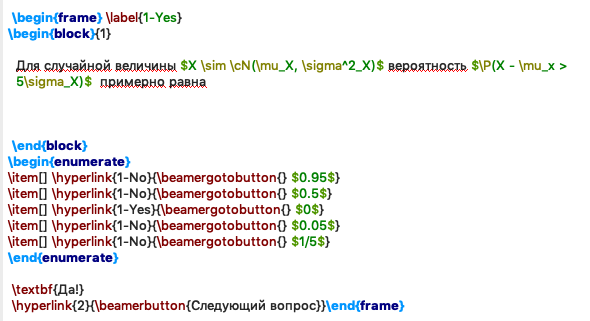
\includegraphics[width=0.8\linewidth]{5.png}}
	\caption{Текст вопроса номер 1 – Ответ правильный.}
	\end{figure}

	\begin{figure}[h!]
	\centering
	\fbox{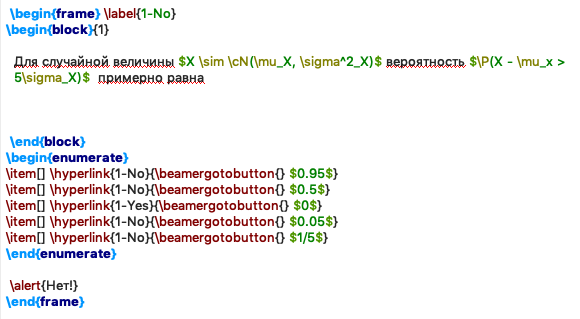
\includegraphics[width=0.8\linewidth]{6.png}}
	\caption{Текст вопроса номер 1 – Ответ неправильный.}
	\end{figure}

	\textbf{Совет:} воспользуйтесь поиском, чтобы быстро переходить из одной части в другую. Удобная метка: <<\form{$\backslash$label\{номер}>>.
	
	\textbf{Совет:} откройте также оригинальный \form{.tex}-файл с заданиями (при наличии), чтобы копировать варианты ответов – это удобно.
	
	\item Типичный вопрос представлен на Рис. 4:
	
	\code{$\backslash$begin\{frame\}} – начало слайда с вопросом. \\
	\code{$\backslash$label\{номер вопроса\}} – метка с номером вопроса. \\
	\code{$\backslash$begin\{block\}\{номер вопроса\}} – заголовок текста вопроса. В качестве заголовка используется номер вопроса. \\
	Далее до \code{$\backslash$end\{block\}} идёт текст вопроса. \\
	Далее между \code{$\backslash$begin\{enumerate\}} и \code{$\backslash$end\{enumerate\}} заключены варианты ответа (в виде списка). Сам текст варианта ответа в каждом пункте списка – это то, что идёт между \code{$\backslash$beamergotobutton\{\}} и закрывающей фигурной скобкой (например, на Рис. 4 в первом варианте ответа текст – \code{\$0.95\$}, на рисунке выделено зелёным). \\
	Слева от \code{$\backslash$beamergotobutton\{\}} в фигурных скобках стоит номер вопроса и указание, верный ли это вариант \code{(номер-Yes)} или нет \code{(номер-No)}. \\
	\code{$\backslash$end\{frame\}} завершает слайд с вопросом.
	
	\item На слайде, указывающем, что выбранный вариант ответа правильный, добавляются два новых элемента после \code{$\backslash$end\{enumerate\}} – это уведомление, что вариант ответа верный и ссылка на следующий вопрос (Рис. 5). На слайде, указывающем, что выбранный варинат ответа неверный, появляется один новый элемент: уведомление, что ответ неверный (Рис. 6). Эти новые элементы редактировать не нужно (за исключением случаев, описанных в <<Корректировке скомпилированного файла>>).
	
	\item Рассмотрим пример возможной проблемы (Рис. 7).
	
	\begin{figure}[h!]
		\centering
		\fbox{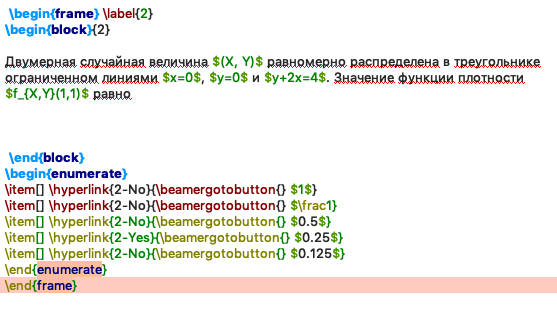
\includegraphics[width=0.8\linewidth]{7.png}}
		\caption{Возможный пример ошибки.}
	\end{figure}

	Проблема: во втором варианте ответа неправильно записана дробь: команда недописана и не хватает закрывающего знака \code{\$}. Верную запись можно посмотреть в оригинальном \form{.tex}-документе (Рис. 8).
	
	\begin{figure}[h!]
		\centering
		\fbox{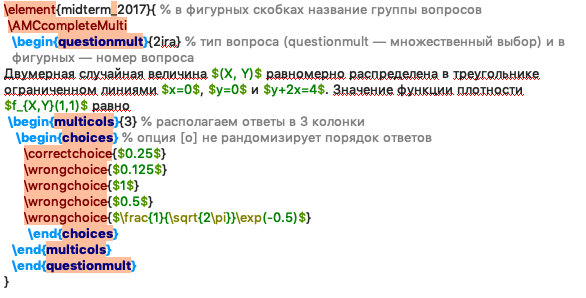
\includegraphics[width=0.8\linewidth]{8.png}}
		\caption{Оригинальное задание.}
	\end{figure}

	Исправленный вариант представлен на Рис. 9.
	
	\begin{figure}[h!]
		\centering
		\fbox{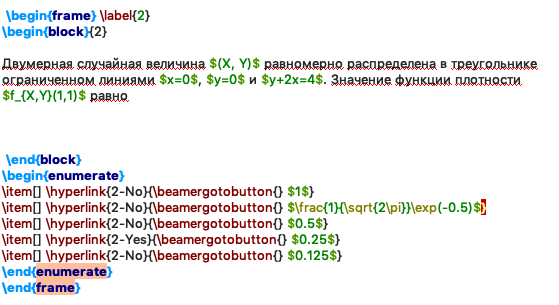
\includegraphics[width=0.8\linewidth]{9.png}}
		\caption{Исправленное задание.}
	\end{figure}

	Не забудьте также внести исправления в слайды с указанием на правильность и неправильность ответа (скопируйте теперь уже правильные варианты и вставьте их вместо вариантов на соответсвующие слайды).
	
	\item Как только будет исправлена последняя ошибка, вы увидите следующий результат (Рис. 10). Не забудьте выставить верное название в преамбуле.
	
	\begin{figure}[h!]
		\centering
		\fbox{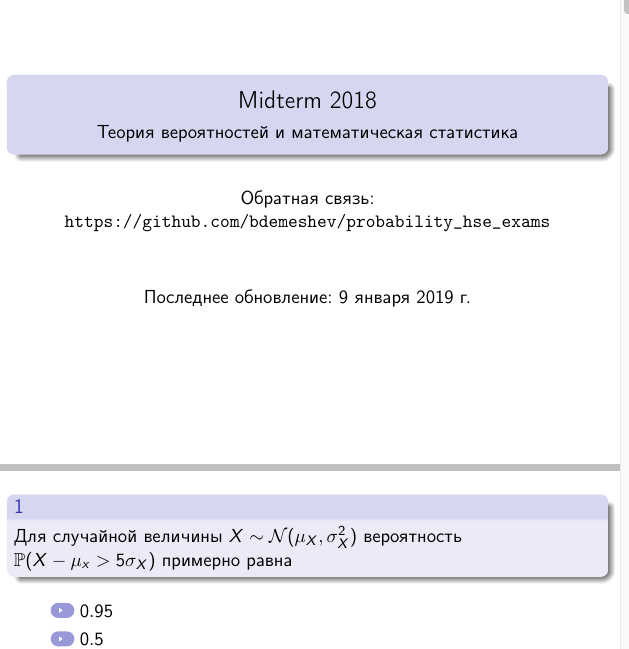
\includegraphics[width=0.8\linewidth]{10.png}}
		\caption{Скомпилированный файл \LaTeX-Beamer.}
	\end{figure}

\end{enumerate}

\section{Корректировка скомпилированного файла}

Просмотрите все слайды с вопросами, чтобы найти ошибки отображения. Не забудьте, что исправления нужно вносить на три слайда, соответствующих одному вопросу. Наиболее частые ошибки:
	\begin{enumerate}
			\item Степени свободы распределений отображются не ниже основного текста, а на одном уровне с ним (то же относится к элементам интегралов, пределов и т.д.) \\
			Решение: потеряны фигурные скобки, заключавшие степени свободы длиной более одного символа. Необходимо их добавить.
			\item В тексте вопроса съехала таблица. \\
			Решение: заключите код таблицы (между командами \code{$\backslash$begin\{tabular\} \ldots $\backslash$end\{tabular\}}) в окружение \code{$\backslash$begin\{center\} \ldots $\backslash$end\{center\}}.
			\item Текст вопроса со всеми вариантами ответа не помещается на слайд. \\
			Решение: удалите команды \code{$\backslash$vskip\{$\cdot$\}} или попробуйте изменить вопрос.
			\item На слайдах с указанием на неправильность или правильность ответа не помещается слово <<Нет!>> или кнопка перехода на следующий слайд. \\
			Решение: вынесите команды, которые задают эти элементы, в заголовок вопроса. Для этого вырежьте их и вставьте в фигурные скобки после \code{$\backslash$begin\{block\}}, после номера вопроса. Должно получиться примерно так, как на Рис. 11.
			\begin{figure}[h!]
				\centering
				\fbox{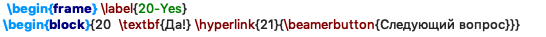
\includegraphics[width=0.8\linewidth]{11.png}}
				\fbox{
\includegraphics[width=0.8\linewidth]{12.png}}
				\caption{Вынесение элементов в заголовок.}
			\end{figure}
			\item В вопросе нет верного варианта ответа. \\
			Решение: измените вопрос, или добавьте на слайд, указывающий на то, что ответ неверный, кнопку перехода на следующий вопрос (скопируйте код кнопки с соответствующего слайда с указанием на верность ответа: всё, что идёт с \code{$\backslash$textbf\{Да!\}} до \code{... Следующий вопрос\}\}}).
	\end{enumerate}

\section{Дополнительно}

\begin{enumerate}
	\item \form{latex2RmdExams.R} – переводит оригинальный \form{.tex}-файл в набор файлов \form{.Rmd}.
	\item \form{RmdExams2latex.R} – переводит набор файлов \form{.Rmd} в формате пакета \form{rexams} в один \form{.tex}-файл (не формата Beamer).
\end{enumerate}
\end{document}